\documentclass[12pt,twocolumn,letterpaper]{article}

\usepackage{cvpr}
\usepackage{times}
\usepackage{epsfig}
\usepackage{graphicx}
\usepackage{amsmath}
\usepackage{amssymb}
\usepackage{esvect}


% Include other packages here, before hyperref.

% If you comment hyperref and then uncomment it, you should delete
% egpaper.aux before re-running latex.  (Or just hit 'q' on the first latex
% run, let it finish, and you should be clear).
\usepackage[breaklinks=true,bookmarks=false]{hyperref}

\cvprfinalcopy % *** Uncomment this line for the final submission

\def\cvprPaperID{****} % *** Enter the CVPR Paper ID here
\def\httilde{\mbox{\tt\raisebox{-.5ex}{\symbol{126}}}}

% Pages are numbered in submission mode, and unnumbered in camera-ready
%\ifcvprfinal\pagestyle{empty}\fi
\setcounter{page}{1}
\begin{document} 

%%%%%%%%% TITLE
\title{Research of Sth}

\author{
Name\\
University of xxx\\
{\tt\small emailaddress}
}
% For a paper whose authors are all at the same institution,
% omit the following lines up until the closing ``}''.
% Additional authors and addresses can be added with ``\and'',
% just like the second author.
% To save space, use either the email address or home page, not both

\maketitle
%\thispagestyle{empty}

%%%%%%%%% ABSTRACT
\begin{abstract}

   
\end{abstract}

%%%%%%%%% BODY TEXT
\section{Introduction}



\section{Related work}

\section{Experiment}
\subsection{Experiment1}


%-------------------------------------------------------------------------

\section{Summary}

\section{Opinion}


\section{Formula symbol}
$\alpha$   $\vec{w}$ 

\[L(\alpha,\omega)=\dfrac{1}{2}||\vec\omega||^2+\sum^n_{i=1} {\alpha_i[z_i(\omega^tx_i+\omega_0)-1]}\]

\[ \min_{\omega_0,\vec\omega} (\max_\alpha \L(\omega_0,\vec\omega,\alpha))\]

\[\dfrac{\partial L(\alpha,\omega)}{\partial{\vec\omega}}=0\]

\[\vec\omega=\sum^n_{i=0}\alpha_i {z_i} \vec{x_i}\]

$\omega_0$ to the function \[ \dfrac{\partial L(\alpha,\omega)}{\partial{\vec\omega_0}}=0 \]

 \[ \sum_{i=0}^n \alpha_i z_i =0 \]

$\xi={\xi_1,\xi_2,...,\xi_n}$

\[f(\vec\omega,\xi)=\dfrac{1}{2} ||\omega||^2+C\sum^n_{i=1} \xi_i\], subject to \[ \forall i, z_i(\vec\omega^t x_i+\omega_0) \geq1-\xi_i, \xi_i \geq 0\]


\section{Figure}

\begin{figure}[h]
    \centering
    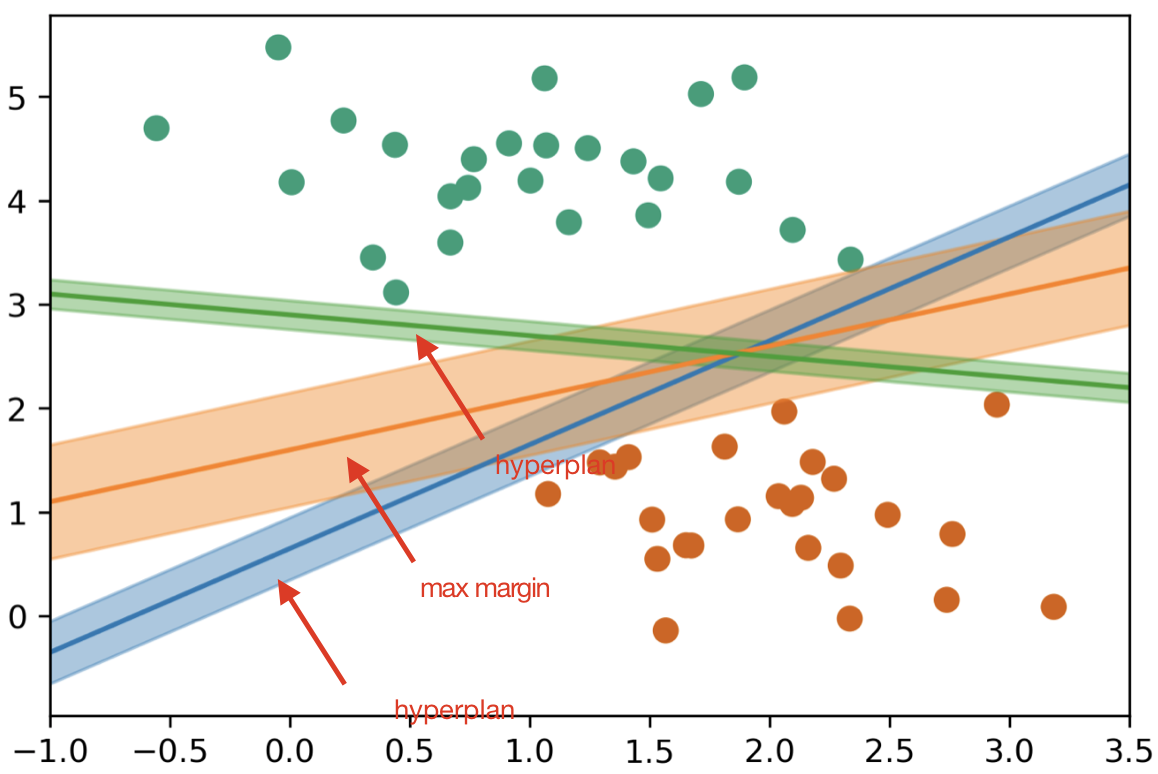
\includegraphics[width=0.4\textwidth]{max_margin.png}
    \caption{hyperplane candidates}
    \label{fig:hyperplane candidates}
\end{figure}


\section{Table}

\begin{table}[!h]
\small

\begin{center}
\begin{tabular}{|p{4cm}|p{4cm}|p{4cm}|}
\hline
Name & Accuracy(C=1)  & b
\\ \hline
Primal & 0.9713 & 3.1171
\\ \hline
Dual & 0.9167 & 1.0092
\\ \hline
\end{tabular}
\end{center}
\end{table}


{\small
\bibliographystyle{ieee}
\bibliography{egbib}
}

\end{document}
